\chapter{Ingeniería Inversa: introducción} \label{cap:capitulo3_I}

En este capítulo se procede a documentar el proceso de ingeniería inversa al que se ha sometido a limitador que puede verse en la imagen {imagen}.

Tal y como se comentó en la sección \ref{sec:contexto}, el punto de partida del proyecto es el estudio y análisis de un limitador funcional y operativo que se encuentra en el laboratorio de \gls{granasat}. Es importante recordar que se dispone del código fuente de este limitador, así como su manual de usuario, el cual nos será de gran ayuda para poder instalarlo correctamente y conocer las capacidades y características generales del producto. De aquí en adelante, se hará referencia al este limitador como \acrshort{LM7}, ya que ese es el nombre técnico del producto.

\begin{figure}
    \centering
    \includegraphics[width=0.9\textwidth]{imagenes/lm7-fotos/lms7.jpg}
    \caption{Limitador LM7.}
	\label{img:lms7_cls}
\end{figure}

\section{Instalación del limitador}

El primer paso a realizar para comenzar el proceso de ingeniería inversa es instalar el equipo. Para ello, se recurre al manual de usuario del equipo, y se siguen las instrucciones de instalación. En la figura \ref{fig:lm7_montaje} se puede observar el esquema de montaje del limitador en un entorno objetivo, es decir, en un establecimiento. En nuestro caso, nuestra entrada no se corresponde a una mesa de mezclas, sino a un ordenador, mediante el cual podremos enviar audio al limitador y comprobar su respuesta.

% Lo manda a otra página
%\begin{figure}[H]
%    \centering
%    \includegraphics[scale=0.25]{figuras/manual7_montaje_trim.pdf}
%    \caption{Esquema conceptual del montaje del \acrshort{LM7}.}
%    \label{fig:lm7_montaje}
%\end{figure}

% Lo encaja en el punto actual del documento
\begin{center}
    \includegraphics[scale=0.6]{figuras/manual7_montaje_trim.pdf}
    \captionof{figure}{Esquema conceptual del montaje del \acrshort{LM7}}
    \label{fig:lm7_montaje}
\end{center}

En la figura superior, podemos observar de izquierda a derecha y de arriba a bajo los siguientes elementos: mesa de mezclas (entrada), micrófono del limitador, limitador de sonido \acrshort{LM7}, altavoces, amplificador (salida).

%\begin{figure}[H]
%    \centering
%    \includegraphics[scale=0.6]{figuras/manual7_trasera_trim2.pdf}
%    \caption{Parte trasera. Conexiones del \acrshort{LM7}.}
%    \label{fig:lm7_trasera}
%\end{figure}
\begin{center}
    \includegraphics[scale=0.55]{figuras/manual7_trasera_trim.pdf}
    \captionof{figure}{Parte trasera. Conexiones del \acrshort{LM7}}
    \label{fig:lm7_trasera}
\end{center}

El sensor S7 (micrófono) es un componente esencial del limitador y forma parte del mismo. Gracias a él, el limitador puede medir la presión acústica en cada momento y actuar en consecuencia. Asimismo, y como se verá más adelante en este documento, será un elemento esencial en la calibración del limitador. El resto del elementos que se muestran en la figura \ref{fig:lm7_montaje} son elementos externos al limitador, y no alteran el funcionamiento del sistema en ninguna forma.

En la figura \ref{fig:lm7_trasera} se pueden observar las principales conexiones del \acrshort{LM7}, las cuales constan de:

\begin{itemize}
    \item Toma de alimentación eléctrica.
    \item Sensor S7 (micrófono) con conector \acrshort{xlr}.
    \item Entradas balanceadas para audio con conectores \acrshort{xlr}.
    \item Salidas balanceadas para audio con conectores \acrshort{xlr}.
    \item Entradas y salidas no balanceadas con conectores \gls{RCA}.
    \item Conector \glsname{rj45} para conexión directa en área local (parte frontal del limitador, no visible en las figuras).
\end{itemize}

Conectamos el micrófono al limitador, así como la entrada y la salida de audio. La salida de audio se conecta a un amplificador de sonido disponible en el laboratorio, y como salida a este sistema de amplificación se conecta un dodecaedro. De forma que podamos tener interacción con el equipo, abrimos el limitador retirando la carcasa metálica exterior, para así poder conectar un teclado y una pantalla a la placa base del equipo. De esta forma descubrimos pro primera vez las entrañas del limitador, y nos encontramos con una tecnología bastante desfasada y un ensamble prácticamente casero. Tal y como podemos ver en la imagen \ref{img:lm7}, el \gls{HW} del limitador se compone de una placa base de tipo industrial, cuyas características de detallan en la tabla \ref{tab:lms7_specs}, un circuito integrado para las entradas y salidas de audio del limitador vistas en la figura \ref{fig:lm7_trasera} y una pequeña caja negra, la cual contiene un relé, y cuya funcionalidad se verá más adelante. Además de esto podemos observar la existencia de una tarjeta de sonido \acrshort{USB} conectada a un puerto \acrshort{USB} de la placa base y cuyas salidas van hacia la caja negra que podemos ver en la imagen. Como dispositivo de almacenamiento interno tenemos un \glsname{CF}, con 1GB de capacidad. En fases posteriores del actual proceso de ingeniería inversa extraeremos esta tarjeta de almacenamiento para acceder a sus archivos, ya que será necesario descubrir o modificar las credenciales de acceso tanto al equipo como al sistema de limitación, pues todas ellas son, por ahora, desconocidas.

\label{img:lms7_open}

Tras revisar todas las conexiones, conectamos el equipo a la corriente eléctrica, y podemos por primera vez ver el equipo en funcionamiento. Mientras arranca el sistema, vemos en la pantalla que el sistema operativo instalado es Debian, una distribución de \gls{GNU/Linux} que se caracteriza por ser minimal. Esta versión en concreto no contiene interfaz gráfica.

Una vez completado el arranque, la pantalla se llena de caracteres que desaparecen rápidamente dando lugar a otros nuevos. De entre lo que es posible leer, se deduce que estos caracteres son datos relativos al limitador (su estado en cada momento, conteniendo lecturas de micrófono y líneas, atenuación aplicada, etc) y que los procesos del limitador vuelcan sus salidas por pantalla a la salida estándar, saturando la terminal principal y dejándola inutilizable. Por tanto, se accede a otra terminal (TTY) mediante la cual podamos trabajar. Esta nueva terminal nos pide usuario y contraseña, las cuales desconocemos.

Continuando con el manual de usuario se descubre que el equipo tiene un servidor web en el cual hay desplegada una interfaz web del limitador, mediante la cual podemos ver su estado, modificar sus configuraciones y obtener informes. Por ello, el próximo y último paso para completar la instalación del limitador es conectarlo a una red interna vía Ethernet, así como conectar y configurar un ordenador adicional mediante el cual podamos acceder, no solo a dicha interfaz web, sino al equipo en sí mediante \acrshort{SSH}.

%\begin{center}
%    \hspace{0cm}
%    \includegraphics[scale=0.7]{imagenes/lms_ip.jpg}
%%    \captionof{figure}{Configuracion \acrshort{IP} del PC adicional}
%%    \captionof{figure}{C}
%    \hspace{2cm}
%    \includegraphics[scale=0.55]{imagenes/lms_ui.jpg}
%%    \captionof{figure}{Interfaz Web de \acrshort{LM7}}
%%    \caption{figure}{C}
%\end{center}

\begin{figure}[ht]
    \begin{minipage}[t]{.45\textwidth}
        \centering
        \includegraphics[width=1\textwidth]{imagenes/interfaz/lms_ip.jpg}
        \caption{Configuración \acrshort{IP} requerida  en el \acrshort{PC} auxiliar.}
        \label{img:lms_ip}
    \end{minipage}
    \hfill
    \begin{minipage}[t]{.45\textwidth}
        \centering
        \includegraphics[width=1\textwidth]{imagenes/interfaz/lms_ui.jpg}
        \caption{Interfaz web del \acrshort{LM7}.}
        \label{img:lms_ui}
    \end{minipage}
\end{figure}

Una vez aplicada la configuración \acrshort{IP} que se muestra en la imagen \ref{img:lms_ip} en el equipo auxiliar, probamos a acceder a la interfaz web de limitador que se encuentra desplegada en la dirección \acrshort{IP}
\href{http://192.168.1.223}{http://192.168.1.223} y vemos por primera vez la aplicación web vista en la imagen \ref{img:lms_ui}. Al entrar en la interfaz web del limitador puede verse la ventana de estado, que informa sobre el estado actual del limitador. Esta interfaz arroja información básica, como:

\begin{itemize}
    \item La presión actual en \glsname{dba} tanto de las líneas como del sensor.
    \item Atenuación aplicada por el limitador en ese instante.
    \item El número de serie del limitador.
    \item El local de instalación
    \item Si el sensor (micrófono) se encuentra conectado o no.
    \item Un gráfico de los últimos 5 minutos de actuación del limitador.
\end{itemize}

En la zona superior derecha, se puede acceder al panel de control y a la sección de obtención de informes. Mediante este panel de control podremos también acceder y modificar la configuración del limitador, aunque para ellos será necesario proveer una clave de acceso válida. En el manual de usuario, se indica que existe un usuario \textit{consultor}, cuya contraseña es a su vez \textit{consultor}. Se trata de un usuario sin privilegios mediante el cual podremos consultar la configuración actual del limitador. Podemos a su vez cerrar sesión mediante el botón \commillas{Cerrar sesión}. Para poder acceder más allá necesitamos averiguar las claves de acceso al limitador.

Para acabar con el proceso de instalación, se comprueba si es posible conectarse mediante \acrshort{SSH} al limitador. Tal y como se esperaba hay conectividad entre los equipos pero necesitamos proporcionar un usuario y una contraseña para acceder al sistema operativo.

Llegados a este punto, el limitador se encuentra instalado y funcionando, pero nuestro control sobre el mismo es completamente nulo ya que no disponemos de las credenciales necesarias para acceder al sistema ni al limitador. Por tanto, procederemos a extraer su dispositivo de almacenamiento, una \glsname{CF}, para investigar desde otro ordenador su contenido y poder encontrar dichas credenciales, dando lugar así al proceso que da nombre a este capítulo, comenzaremos con el proceso de Ingeniería Inversa.

\subsection{Resumen} \label{cap1:sec1:resumen}

Como resumen a esta sección, se han realizado las siguientes acciones:

\begin{enumerate}
    \item Se ha conectado el limitador \acrshort{LM7} a corriente y se han conectado a él un monitor (interfaz VGA) y un teclado (interfaz PS/2).
    \item Se ha instalado un \acrshort{PC} auxiliar con el sistema operativo \gls{WINDOWS} 10.
    \item Se han conectado los dos equipos mediante Ethernet, usando un Switch de la marca OvisLink, con la configuración de red vista en la imagen \ref{img:lms_ip}.
\end{enumerate}

Como consecuencia de dichas acciones, tenemos los dos equipos conectados en red, por lo que se puede acceder al limitador desde el equipo auxiliar mediante \acrshort{SSH}, aunque desconoce el usuario y contraseña del sistema.

\section{Extracción de credenciales} \label{lm7-credenciales}

Para conseguir el acceso al sistema limitador, extraemos el dispositivo de almacenamiento y lo exploramos en otro ordenador mediante un adaptador. Explorando el sistema de archivos se descubre la existencia de un directorio peculiar dentro del directorio \textit{/var} en el nivel principal de la estructura de directorios de Linux.

\begin{center}
    \includegraphics[scale=0.5]{figuras/unix_filesystem_hierarchy.pdf}
    \captionof{figure}[Estructura de directorios de un sistema GNU/Linux]
    {
        Estructura de directorios de un sistema \gls{GNU/Linux} \\
        Fuente : \cite{wikipedia}
%        Fuente: \href{https://upload.wikimedia.org/wikipedia/commons/f/f3/Standard-unix-filesystem-hierarchy.svg}{Wikipedia}
    }
    \label{fig:dirs_linux}
\end{center}

\subsection{Credenciales del limitador}

Dentro de esta carpeta denominada \textit{slr/} encontramos rápidamente un fichero llamado \textbf{\textit{users.auth}}, con usuarios, claves y permisos. Estas credenciales no son las del sistema operativo que corre sobre la máquina, sino las de los usuarios que tienen acceso a la configuración del limitador, es decir, son los usuarios y contraseñas necesarios para acceder a la aplicación web del limitador (imagen \ref{img:lms_ui}), así como los permisos de estos usuarios sobre la configuración del limitador.

\begin{shaded}
%    \textbf{\textit{slr/}}
    \noindent
    El directorio \textbf{slr/} será de gran importancia en el ámbito del proyecto, ya que en este directorio se almacenarán la gran mayoría de ficheros relacionados con el limitador: datos de configuración, información de usuarios, ficheros de sonido, e incluso ficheros que funcionarán a modo de variables globales del limitador. Conforme se vaya avanzado en el documento se irá describiendo y explicando cada uno de estos ficheros.
    \par
    \noindent
    El nombre del directorio se deduce que es un acrónimo de \textit{\textbf{S}ound\textbf{L}imiter\textbf{R}ecords}.
\end{shaded}

Para nuestra sorpresa, se descubre que los datos no sólo están almacenados en un fichero de texto plano, sino que tampoco se encuentran cifrados. Cada una de las líneas del fichero define un usuario con los siguientes campos:

\begin{itemize}
    \item \acrshort{dni}.
    \item Nombre.
    \item Contraseña.
    \item Gestor de usuarios (si puede crear, modificar o eliminar usuarios).
    \item Gestor de configuración (si puede modificar la configuración del limitador).
    \item Fecha del alta del usuario en el sistema.
\end{itemize}

En el listado \ref{lst:usersAuth} pueden verse claros ejemplos del patrón definido justo sobre estas líneas. Adicionalmente, existen en el fichero otras líneas que no siguen este patrón y definen otros patrones nuevos. Ejemplos de estas líneas son las que encontramos en la línea 4 y 14 del listado \ref{lst:usersAuth}. Estas líneas definen el modo de acceso al limitador y la eliminación de un usuario en el sistema, respectivamente, así como la marca de tiempo de la acción que dio origen a la inserción de esas líneas en el fichero.

Para confirmar el descubrimiento de las credenciales del limitador se comprueban algunos de los usuarios y claves encontradas en la interfaz web del limitador, con resultado satisfactorio. Se consigue por tanto el acceso a la configuración del limitador y tenemos ahora el control sobre él, aunque seguimos sin disponer de control sobre el sistema operativo sobre el que corre.\newline

\begin{lstlisting} [language=HTML, label={lst:usersAuth}, caption={Contenido del fichero \textit{users.auth}}]
    dni=*lm7-passwordUser&name=Password user&password=\t****&userManager=1&configManager=1&time=2012/05/11-11:48:36
    dni=*lm7-remoteUser&name=Remote system user&password=\t****&userManager=0&configManager=0&time=2012/05/11-11:48:36
    dni=consultor&name=Consultor&password=consultor&userManager=0&configManager=0&time=2012/05/11-11:48:36
    key=authMethod&value=onlyPassword&time=2012/08/30-05:35:16
    dni=E19578186&name=NOISEOFF&password=COCHA012015&userManager=1&configManager=1&time=2015/06/25-23:07:38
    dni=E19578186&name=NOISEOFF&password=COCHA012015&userManager=1&configManager=1&time=2015/06/25-23:08:13
    dni=E19578186&name=NOISEOFF&password=01COCHA2015&userManager=1&configManager=1&time=2015/06/26-14:55:51
    key=authMethod&value=onlyPassword&time=2015/06/26-14:57:58
    dni=E19578186&name=NOISEOFF&password=COCHA0130115&userManager=1&configManager=1&time=2016/09/20-19:14:48
    dni=E19578186&name=NOISEOFF&password=COCHA0130115&userManager=1&configManager=1&time=2016/09/20-19:16:21
    key=authMethod&value=onlyPassword&time=2016/09/20-19:16:50
    dni=E19578186&name=NOISEOFF&password=cocha0130115&userManager=1&configManager=1&time=2017/01/02-12:08:33
    dni=44289989Q&name=NOISEOFF&password=cocha0130115&userManager=1&configManager=1&time=2017/01/02-12:10:05
    dni=E19578186&deleted=1
    key=authMethod&value=onlyPassword&time=2017/01/02-12:12:01
    dni=44289989Q&name=NOISEOFF&password=cocha0130115&userManager=1&configManager=1&time=2017/01/05-09:50:40
    key=authMethod&value=onlyPassword&time=2017/01/05-09:52:03
\end{lstlisting}

\subsection{Credenciales del sistema operativo}

Para obtener el control sobre el sistema operativo es necesario disponer de un usuario y contraseña válidos de forma que podamos acceder a él mientras el equipo está en funcionamiento.

Del sistema operativo sabemos que es \gls{debian}, una distribución \gls{GNU/Linux}, por tanto, se investiga dónde almacena este sistema sus usuarios. Son datos estáticos así que deben encontrase almacenados en alguna parte dentro del sistema de archivos contenidos en el disco, el cual, recordamos, tenemos conectado a otro ordenador mediante un adaptador \acrshort{USB}.

A través de la consulta de foros
 \href{https://www.cyberciti.biz/faq/where-are-the-passwords-of-the-users-located-in-linux/}{(cyberciti.biz)} y manuales \href{https://www.debian.org/doc/manuals/system-administrator/ch-sysadmin-users.html}{(Debian.org)} en línea, descubrimos que los ficheros que necesitamos son \textbf{/etc/passwd} y \textbf{/etc/shadow}. Aunque ambos contienen información crítica sobre los usuarios y sus permisos, existen pequeñas diferencias. En resumen, mientras que \textbf{/etc/passwd} almacena información mayormente relativa al usuario, \textbf{/etc/shadow} contiene las claves de usuario (encriptadas) e información relacionada a ellas, no al usuario.

%El fichero \textbf{/etc/shadow} contiene una entrada por línea para cada uno de los usuarios listados en el fichero \textbf{/etc/passwd}. Las claves están compuestas por una serie de campos, separados por dos puntos (:), y son de la siguiente manera:

Las contraseñas encriptadas y otra información relacionada, como la información de caducidad de la contraseña, se almacenan en el fichero \textbf{/etc/shadow}. Este fichero contiene una entrada por línea por cada uno de los usuarios listados en el fichero \textbf{/etc/passwd}. Cada una de estas entradas están compuestas por una serie de campos separados por dos puntos (:), y generalmente, sigue este patrón.

\begin{center}
    \includegraphics[scale=0.5]{figuras/shadow.pdf}
    \captionof{figure}{Estructura de las claves en el fichero \textbf{/etc/shadow}}
    \label{fig:shadow}
\end{center}

\begin{enumerate}
    \item Nombre de usuario.
    \item Contraseña encriptada (\textbf{hash}). Sigue el formato \textbf{\textdollar id\textdollar salt\textdollar hash}. El campo \textbf{\textdollar id} representa el algoritmo usado:
        \begin{enumerate}
           \item \textbf{\textdollar 1\textdollar } es MD5.
           \item \textbf{\textdollar 2a\textdollar} es Blowfish.
           \item \textbf{\textdollar 2y\textdollar} es Blowfish.
           \item \textbf{\textdollar 5\textdollar } es SHA-256.
           \item \textbf{\textdollar 6\textdollar } es SHA-512.
        \end{enumerate}
    \item Días desde que se cambió la contraseña, contando desde el 1 de enero de 1970.
    \item Días tras los cuales la contraseña debe ser cambiada.
    \item Días de antelación a la expiración de la contraseña en los que se avisa al usuario.
    \item Días tras los cuales se desactiva una cuenta cuya contraseña está caducada.
\end{enumerate}

\begin{shaded}
    \noindent
    Una contraseña \textbf{hash} no es más que una cadena de caracteres única, la cual es resultado de la ejecución de un algoritmo de encriptación, dada otra cadena de caracteres como entrada. Esta contraseña \textbf{hash} es la que se almacena en el sistema, y no la contraseña original. Durante el proceso de inicio de sesión, se comprueba el \textbf{hash} de la contraseña insertada por el usuario y la contraseña \textbf{hash} almacenada, verificando así la integridad de la misma.
\end{shaded}

Abrimos el fichero \textbf{/etc/shadow} y encontramos la información que necesitamos. La imagen \ref{img:shadow} muestra el contenido de este fichero.

\begin{center}
    \includegraphics[scale=0.25]{imagenes/shadow.png}
    \captionof{figure}[Contenido del fichero /etc/shadow del LM7]
    {Contenido del fichero \textbf{/etc/shadow} del \gls{LM7}}
    \label{img:shadow}
\end{center}

Los usuarios que nos interesan son \textbf{root} y \textbf{lmuser}. Ambas contraseñas se han cifrado usando el algoritmo SHA-512, ya que su primer campo es \textdollar 6\textdollar. En un primer intento se modifica el fichero y se eliminan los campos que contienen la contraseña \textit{Hash}, con la intención de forzar el inicio de sesión sin la necesidad de contraseña (contraseña vacía). Sin embargo, este enfoque no produce el resultado esperado y se busca otra solución. \\ Como conocemos tanto el formato de las entradas de este fichero como el algoritmo de cifrado utilizado, el segundo enfoque será sustituir estas claves \textit{Hash} con otras nuevas, generadas por nosotros. Generamos una nueva contraseña usando la utilidad \gls{openssl}.\newline

\begin{lstlisting}[language=bash, label={lst:openssl}, caption={Generación de Hash usando cifrado SHA-512}]
    $~ openssl passwd -6 <cadena>
\end{lstlisting}

La ejecución del comando \ref{lst:openssl} nos genera una clave Hash única para la cadena que le proporcionemos como entrada. La opción -6 indica que debe usarse el algoritmo de cifrado SHA-512. Para más información sobre este comando y sus opciones puede consultarse la documentación oficial \cite{openssl}.

Una vez cambiadas las contraseñas por las que hemos generado, re-instalamos el \glsname{CF} en la placa base del limitador y se procede a encenderlo para comprobar que podemos acceder al sistema con las nuevas credenciales. Tras finalizar el arranque se verifica que el inicio de sesión con ambos usuarios es satisfactorio, y que por tanto, se tiene control sobre el sistema operativo. La conexión al equipo mediante \acrshort{SSH} también funciona correctamente usando las nuevas contraseñas. Anteriormente, se ha comprobado que la configuración \acrshort{SSH} del sistema permite la conexión mediante el usuario \textit{root}. Para ello se comprueba que en el fichero de configuración en la ruta /etc/sshd\textunderscore conf contiene la directiva \textit{PermitRootLogin} y que su valor es YES. Tras comprobar el fichero, se verifica que la directiva existe y está configurada correctamente. Este no es el valor por defecto, por lo tanto ha tenido que ser activado con anterioridad. Además, se añade la siguiente directiva para garantizar el acceso a los usuario \textit{root} y \textit{lmuser}: \newline

\begin{lstlisting}[nolol, language=XML, label={lst:confSSH}, caption={Directiva del fichero}]
    AllowUsers root lmuser
\end{lstlisting}

\section{Especificaciones del sistema}

El primer paso para comenzar a investigar el equipo es descubrir ante que tipo de hardware nos enfrentamos. En secciones anteriores (imagen \ref{img:lms7_open}) se mostró el hardware del limitador bajo estudio, y se comentó brevemente sus características. En esta sección, se va a realizar un análisis más profundo sobre las capacidades y características hardware del sistema:

Nos encontramos antes un equipo en el que se ha montado una placa base de tipo industrial, en la que vienen integrados todos los recursos hardware necesarios para correr un sistema operativo. En la siguiente tabla pueden verse los componentes básicos con los que cuenta el sistema:

\begin{table}[h]
    \centering
    \begin{tabular}{|>{\columncolor[HTML]{ECF4FF}}l |l|}
        \hline
        Placa base     & ALIX-1E                    \\ \hline
        Procesador     & AMD Geode LX               \\ \hline
        Memoria        & 128/256MB SDRAM            \\ \hline
        Almacenamiento & CompactFlash 1GB           \\ \hline
        Interfaces     & 4x\glsname{USB}, 1x\glsname{VGA}, 1x\glsname{LPT}, 2x\glsname{COM} \\ \hline
        Conectividad   & Ethernet                   \\ \hline
        Dimensiones    & 17x17cm                    \\ \hline
    \end{tabular}
    \caption{Especificaciones hardware del \gls{LM7}}
    \label{tab:lms7_specs}
\end{table}

Como componentes que no forman parte de la placa base, tenemos una tarjeta de sonido USB conectada a uno de los puertos y un circuito integrado para las entradas y salidas de audio, conectado a la placa base mediante su puerto serie.

\begin{figure}
    \centering
    \includegraphics[width=0.9\textwidth]{imagenes/lm7-fotos/lms7-comps.jpg}
    \caption{Limitador LM7 y sus componentes montado en una placa base ALIX-1B.}
%	\label{img:alix1b}
\end{figure}

\begin{center}
    \includegraphics[scale=0.75]{imagenes/alix1b.jpg}
    \captionof{figure}{Imagen de una placa base ALIX-1B \cite{alix}}
    \label{img:alix1b}
\end{center}

\section{Análisis del rendimiento} \label{sec:lms7-performance}

Tal y como se comentó en la primera sección de este capítulo, el ordenador auxiliar que se ha instalado en el laboratorio, y en red como el \gls{LM7}, tiene \gls{WINDOWS} 10 como sistema operativo. Para facilitar el acceso remoto mediante \acrshort{SSH} al equipo limitador, se hace uso de clientes \acrshort{SSH}. En la tabla \ref{tab:gestoresSSH} se lista el cliente usado tanto en Windows 10 como en Linux.

% Please add the following required packages to your document preamble:
% \usepackage{graphicx}
\begin{table}[h]
    \centering
    \begin{tabular}{|l|l|}
        \hline
        \rowcolor[HTML]{ECF4FF}
        Sistema Operativo & Cliente SSH   \\ \hline
        Linux             & Snowflake SSH \\ \hline
        Windows           & MobaXterm     \\ \hline
    \end{tabular}
    \caption{Clientes \acrshort{SSH} utilizados en el proyecto.}
    \label{tab:gestoresSSH}
\end{table}

Estos clientes aportan ciertas ventajas, como por ejemplo:

\begin{itemize}
    \item Permiten guardar los datos de acceso a equipos remotos. Una conexión \acrshort{SSH} a otro equipo se resume en hacer click sobre un botón.
    \item Proporcionan una interfaz gráfica.
    \item Disponen de un navegador de archivos.
    \item Monitorizan el sistema remoto, lo que nos permite analizar el uso de recursos (disco, memoria, \acrshort{CPU} y red) en tiempo real.
\end{itemize}

Tras configurar el cliente \acrshort{SSH}, se lanza una conexión remota al \gls{LM7}. Los datos de monitoreo muestran una alta tasa de utilización del \acrshort{CPU}, en torno al 85-100\% (ver imágenes \ref{img:lms_ps1} y \ref{img:lms_ps2}). Indudablemente, el hecho de que el \acrshort{CPU} disponga de una único núcleo es significativo, sin embargo, se procede a identificar los procesos en funcionamiento que pertenecen al limitador. Para ello, se recurre al código fuente del limitador, en concreto al fichero \gls{makefile}, el cual se encarga de compilar los distintos ejecutables (a los que llamaremos \textbf{módulos}) y de moverlos al directorio raíz del sistema: \textbf{/bin}. Al colocar los programas en esta carpeta, se pueden lanzar de forma global, es decir, sin especificar su ruta.

\begin{figure}[ht]
    \begin{minipage}[b]{.45\textwidth}
        \centering
        \includegraphics[width=1\textwidth]{imagenes/lm7_ps[1].png}
        \caption{Procesos del LM7 [1/2]}
        \label{img:lms_ps1}
    \end{minipage}
    \hfill
    \begin{minipage}[b]{.45\textwidth}
        \centering
        \includegraphics[width=1\textwidth]{imagenes/lm7_ps[2].png}
        \caption{Procesos del LM7 [2/2]}
        \label{img:lms_ps2}
    \end{minipage}
\end{figure}

El fichero \gls{makefile} nos proporciona una lista de nombres de procesos a buscar. Listamos los procesos activos con la orden \textbf{ps}. El comando completo así como el resultado devuelto pueden observarse en las captura de pantalla \ref{img:lms_ps1} y \ref{img:lms_ps2}. Las opciones pasadas al invocar al comando \textbf{ps} permite mostrar no solo los procesos en activo, sino también las relaciones jerárquicas que existen entre ellos. La mayoría de los procesos del limitador son fácilmente detectables incluso en el supuesto de que se conocieran sus nombres con anterioridad. Los procesos relativos al limitador se encuentran remarcados en rojo, y se puede apreciar el detalle de que todos ellos tiene como proceso padre  a \textbf{init}, con \acrshort{PID} 1. Podemos ver esta información en la primera columna de la tabla, \acrshort{PPID}. Esto significa que los procesos del limitador son lanzados automáticamente al arrancar el sistema. Se profundizará sobre esto en la sección \ref{sec:lms7-init}, donde se explicará proceso de arranque del LM7.

Los procesos que componen en limitador se verán con profundidad en la sección \ref{sec:lm7-procesos}, pero antes, se presentará y estudiará la interfaz web del limitador en su totalidad (ya se presentó la sección principal con la imagen \ref{img:lms_ui}), mediante la que podemos configurarlo y visualizar las lecturas de los sensores y la atenuación aplicada en cada momento.

\section{Interfaz web}

La interfaz web del limitador se encuentra desplegada en un servidor \gls{apache}, y está programada usando PHP, \acrshort{CSS}, HTML y Javascript. En la tabla \ref{tab:lm7_lamp_specs} puede consultarse un análisis más detallado de las tecnologías usadas en la interfaz web.

% Please add the following required packages to your document preamble:
% \usepackage[table,xcdraw]{xcolor}
% If you use beamer only pass "xcolor=table" option, i.e. \documentclass[xcolor=table]{beamer}
\begin{table}[h]
    \centering
    \begin{tabular}{|l|l|}
        \hline
        \rowcolor[HTML]{ECF4FF}
        \multicolumn{1}{|c|}{\cellcolor[HTML]{ECF4FF}\textbf{Tecnología}} & \multicolumn{1}{c|}{\cellcolor[HTML]{ECF4FF}\textbf{Versión}} \\ \hline
        Sistema Operativo                                                 & Debian 4.3.5                                                  \\ \hline
        Servidor Web                                                      & Apache 2.2.16                                                 \\ \hline
        PHP                                                               & 5.5.3                                                         \\ \hline
    \end{tabular}
    \caption{Especificaciones del servidor web del \gls{LM7}}
    \label{tab:lm7_lamp_specs}
\end{table}

El estudio del la interfaz representa un aspecto clave en el proceso de ingeniería inversa en el que nos encontramos. La interfaz web arroja una gran cantidad de información mediante la cual somos capaces no sólo de comprender qué hace el sistema, qué datos almacena y como los representa y exporta, sino que también nos permite generar un conjunto de requisitos funcionales, no funcionales y de datos que nuestro proyecto deberá satisfacer, y como mínimo, debe hacerlo tan bien (o mal) como el sistema estudiado (requisitos de calidad). Por otra parte, será una guía y un recurso al cual recurriremos una y otra vez a lo largo de este proyecto. En definitiva, la interfaz web nos permite, de un vistazo, comprender el sistema y sus capacidades.

\subsection{Imágenes}

En esta subsección se va a presentar las interfaz web en imágenes de forma que el lector pueda ver la interfaz web por sí mismo, aunque de forma estática. Todas estas imágenes has sido extraídas del manual de usuario del limitador \acrshort{LM7}.

%\begin{figure}[H]
\begin{figure}[ht]
    \centering
    \includegraphics[width=0.75\textwidth]{imagenes/interfaz/Interfaz_0.png}
    \caption{Vista principal. Estado del limitador.}
\end{figure}

%\begin{figure}[H]
\begin{figure}[ht]
    \centering
    \includegraphics[width=0.75\textwidth]{imagenes/interfaz/Interfaz_1_menu.png}
    \caption{Panel de control antes de identificación.}
\end{figure}

%\begin{figure}[H]
\begin{figure}[ht]
    \centering
    \includegraphics[width=0.75\textwidth]{imagenes/interfaz/Interfaz_2_menu_acceso.png}
    \caption{Panel de control después de identificación}
\end{figure}

%\begin{figure}[H]
\begin{figure}[ht]
    \centering
    \includegraphics[width=0.75\textwidth]{imagenes/interfaz/Interfaz_3_aislamiento.png}
    \caption{Aislamiento.}
\end{figure}

%\begin{figure}[H]
\begin{figure}[ht]
    \centering
    \includegraphics[width=0.75\textwidth]{imagenes/interfaz/Interfaz_4_festivos_0.png}
    \caption{Normativa [1/2].}
\end{figure}

%\begin{figure}[H]
\begin{figure}[ht]
    \centering
    \includegraphics[width=0.75\textwidth]{imagenes/interfaz/Interfaz_4_festivos_1.png}
    \caption{Normativa [2/2].}
\end{figure}

%\begin{figure}[H]
\begin{figure}[ht]
    \centering
    \includegraphics[width=0.75\textwidth]{imagenes/interfaz/Interfaz_5_datos_local.png}
    \caption{Datos del local.}
\end{figure}

%\begin{figure}[H]
\begin{figure}[ht]
    \centering
    \includegraphics[width=0.75\textwidth]{imagenes/interfaz/Interfaz_6_usuarios_0.png}
    \caption{Gestión de usuarios.}
\end{figure}

%\begin{figure}[H]
\begin{figure}[ht]
    \centering
    \includegraphics[width=0.75\textwidth]{imagenes/interfaz/Interfaz_7_calibrar_0.png}
    \caption{Calibración [1/2].}
	\label{img:lms7-calibrate}
\end{figure}

%\begin{figure}[H]
\begin{figure}[ht]
    \centering
    \includegraphics[width=0.75\textwidth]{imagenes/interfaz/Interfaz_7_calibrar_1.png}
    \caption{Calibración [2/2].}
\end{figure}

\clearpage
\subsection{Análisis técnico}

En esta subsección profundizamos un poco más en la interfaz web recurriendo a su código fuente. Bajamos por tanto un escalón importante a nivel de abstracción. Por razones obvias, no se va a incluir la totalidad del código de la interfaz web del limitador en esta subsección, sino que se va a realizar un análisis técnico del mismo, destacando las cualidades o deficiencias más importantes que se han detectado y presentando bloques de código que den soporte al análisis y ayuden a comprenderlo.

%La interfaz web se compone de XX ficheros, los cuales comoponen un total de YY líneas de código y se dividen en un total de 11 directorios, aunque como se verá luego no todos ellos contienen código. Hay que tener en cuenta que en este recuento se incluyen imágenes, librerías estáticas (tanto de JS como de CSS) y código etiquetado como \enquote{antiguo}. De hecho, la carpeta \enquote{old} tiene no una, sino dos versiones preliminares de la interfaz web. Además, en la carpeta simple se

Como se ha comentado en la introducción a esta sección, el código de la interfaz web se compone de código PHP, HTML, CSS y JS. Parte del código CSS y JS corresponde a librerías estáticas, descargas y usadas por el proyecto, como por ejemplo \href{https://jquery.com/}{jQuery}, y su plugin \href{https://nathansearles.github.io/slidesjs/}{SlideJS}, \href{https://dygraphs.com/}{dygraphs} o \href{https://github.com/arv/explorercanvas}{ExCanvas}. Estas librerías se usan de forma extensiva para construir toda la parte reactiva y asíncrona de la interfaz, como las acciones lanzadas mediante la pulsación de botones, el envío de datos al servidor y la actualización de datos en la interfaz, sin necesidad de recargar la página; para ello, se hace uso de AJAX. Las dos últimas librerías se usan concretamente para la generación de gráficos, en este caso, la gráfica principal que muestra las lecturas de los sensores y la atenuación aplicada por el limitador en cada momento.

En el esquema \ref{lst:lm7-www-treeview} podemos observar la estructura de la carpeta \verb|www| dentro del código fuente del limitador, la cual contiene el código de la interfaz web. Por simplicidad, se han omitido algunos los ficheros no esenciales, ya que el listado sería demasiado extenso y la intención es mostrar la estructura y organización del proyecto que materializa la aplicación web, así como describir brevemente el propósito y responsabilidad de cada fichero. Para generar esta representación del directorio y su contenido se ha utilizado la herramienta \acrshort{GIO}, disponible en distribuciones de Linux.\newline

\begin{lstlisting}[label={lst:lm7-www-treeview}, caption={Estructura de directorios y ficheros de la interfaz web}]
    # gio tree .../lms.7/lms/www

    file:///lms.7/lms/www
    |-- access.php                              # Gestión de usuarios, sesiones y permisos
    |-- authPart-ExtendedNormative.php
    |-- calibrationControl.lib.php
    |-- config.xml
    |-- configFail.inc
    |-- configuration.php                       # Definición de variables globales
    |-- css/
    |-- fonts/
    |-- functions/                              # Scripts AJAX
    |   |-- calibrate.php                       # Actualizador de calibración
    |   |-- network.php                         # Controlador de configuración de red
    |   |-- pink.php                            # Control de la emisión de ruido rosa
    |   |-- restart.php
    |   |-- soundControl.php
    |   |-- status.php                          # Consulta el estado del limitador
    |   |-- updateCnfg.php                      # Actualizador de configuración
    |   |-- updateDataCu.php                    # Actualizador de datos del local
    |   |-- updateExtendedNormative.php         # Actualizador de la normativa
    |   |-- updatePwd.php                       # Actualizador de contraseña
    |   |-- updateTime.php                      # Actualizador de fecha y hora
    |   `-- validateUserCode.php
    |-- help.png
    |-- images/
    |-- index.php                               # Controlador principal
    |-- jquery.css
    |-- js/                                     # Librerías JS (jQuery, dygraph, slide, excanvas..)
    |-- leftEqualizer.php                       # Template de ecualizador izquierdo (HTML, CSS, JS, PHP)
    |-- login.php          alibra                     # Script de login (PHP)
    |-- logoPagina.png
    |-- logs.php                                # Logger
    |-- manual.php
    |-- manual3.pdf                             # Manual de usaurio de los limitadores serie 3
    |-- manual7.pdf                             # Manual de usaurio de los limitadores serie 7
    |-- new/
    |-- old/                                    # Versiones antiguas de la aplicación web
    |   |-- www/
    |-- reportOutputTest.html
    |-- reports/                                # Generación y exportación de informes
    |   |-- CreateReport.php
    |   |-- PhpDataGetter.php
    |   |-- data.php
    |   |-- data.xml.php
    |   |-- engine.php
    |   |-- engine_render.php
    |   |-- engine_render2.php
    |   |-- engine_render3.php
    |   |-- getReport.php
    |   |-- images/
    |   |-- index.php
    |   |-- logoReports.png
    |   |-- reportContent.php
    |   |-- reportError.html
    |   |-- reportError.php
    |   |-- reportHasNoScreenableOutput.html
    |   |-- reportHelp.html
    |   |-- reportTemp -> /tmp/templateTempDirectory/
    |   |-- saveCreatedReport.php
    |   |-- testEngine.php
    |   |-- testSaved.php
    |   `-- tmp -> /tmp
    |-- rightEqualizer.php                      # Template de ecualizador derecho (HTML, CSS, JS, PHP)
    |-- scripts.js                              # Código JS global (la mayoría está embebido en los .php)
    |-- simple/                                 # Versión simplificada de la web
    |-- smallInfoPanel.php
    |-- statusPart.php
    |-- style-Blue.css
    |-- style.css
    |-- tabAuth.php                             # Template del panel superior si se está autenticado
    |-- tabAuthRegister.php                     # Template del panel superior para el registro
    |-- tabNormal.php                           # Template del panel superior si NO se está autenticado
    |-- templateMng.php
    |-- tests/
    |-- tractis/                                # DNI-e (no usado)
    `-- users.php                               # Gestión de usuarios (deprecated en favor de access.php)
\end{lstlisting}

La página web se genera de forma dinámica mediante PHP, en función de:
\begin{itemize}
    \item Tipo de usuario (roles y permisos).
    \item Si el usuario ha iniciado sesión o no.
    \item Tipo de sistema (registrador o limitador).
    \item Los datos (actualización asíncrona).
\end{itemize}

La generación de código dinámico se basa en la renderización condicional de bloques de código fuente, así como la inclusión (a veces también condicional) de otros ficheros con extensión PHP. Es importante destacar que en este aspecto \textbf{no se hace uso de ninguna herramienta} que ayude a gestionar la generación dinámica del código, como puede ser un \textbf{gestor de plantillas} como Twig. Esto, junto con el\textbf{ uso de código en varios lenguajes} (PHP, JS, HTML y CSS) de manera simultánea en el mismo fichero e incluso \textbf{en el mismo bloque de código} hace que el código de la aplicación web sea \textbf{altamente complejo y difícil} de leer, entender y sobretodo, \textbf{de mantener}. Podemos observar un ejemplo claro de esto en el siguiente extracto de código, perteneciente al fichero \textit{tabAuth.php}:\newline

\begin{lstlisting}[
    language=HTML,
    label={lst:lm7-www-code-mixed},
    caption={Código HTML, CSS, JS y PHP usado de forma conjunta}
]
    ...
    <div id="chTime" title="Cambio de hora">
    <p style="font-size:bigger; font-weight:bold;">Cambio de hora del sistema</p>

    <p>Hora actual <span id="chTime_actualTime"></span></p>
    <p>
    <form id="chTime_form">
    Nueva hora <input type=text id="chTime_new" name="chTime_new" style="width:120px" value="" <?php if (!$configurator){ echo( 'disabled="disabled"'); }?> ></input>
    </form>
    </p>
    <br/>
    <img src="images/alert.png"> Recuerde: El sistema actualizar&aacute; autom&aacute;ticamente la hora al estar conectado a internet.
    <table width=100%>
    <tr>
    <td>
    <input style="float:right" type="button" value="Cerrar" id="" class="bt_register" onclick="javascript:$('#chTime').dialog('close');" />
    </td>
    <td align=right>
    <?php if ($configurator){ ?>
        <input style="float:right" type="button" value="Ok" id="" class="bt_register" onclick="javascript:ChTime_UpdateClock();" />
        <?php } ?>
    </td>
    </tr>
    </table>
    </div>
    <script>
    $('#chTime_new').datetimepicker({
        dateFormat: 'yy/mm/dd'
    });
    </script>

    <script>
    function ChTime_UpdateClock() {
        $.ajax({
            data: $("#chTime_form").serialize(),
            type: "POST",
            dataType: "json",
            url: "functions/updateTime",
            success: function(data) {
                alert("Hora actualizada");
            }
        });
    };
    </script>
    ...
\end{lstlisting}

El código \ref{lst:lm7-www-code-mixed} ha sido ligeramente indentado y reestructurado para mejorar su comprensión, sin embargo, al problema que supone desarrollar código como el que acabamos de ver, hay que sumar una indentación prácticamente inexistente, la ausencia casi total de comentarios y la prolongación de líneas de código por encima de los 100 caracteres de longitud.

Tan solo los ficheros \textit{tabNormal.php, tabAuth.php} y \textit{tabAuthRegister.php} suman un total de 3000 líneas de código, por lo que la complejidad del código crece rápidamente en un proyecto de estas características cuando se siguen malas prácticas como las que se acaban de ver. Además de las claras deficiencias del código en sí, la interfaz web está \textbf{fuertemente acoplada} al sistema operativo y al software del limitador, ya que la comunicación IU-Limitador se realiza exclusivamente mediante ficheros o mediante la invocación directa de procesos / servicios del limitador que se ejecutan sobre el sistema operativo. Estos dos procedimientos de comunicación se verán en detalle en la siguiente sección.

En definitiva, la complejidad del código debido a malas prácticas y las complejidades técnicas que supone el uso de PHP 5 a la fecha de la redacción de este documento provocan que no sea factible la reutilización de la aplicación web, y por tanto, queda exclusivamente como objeto de estudio y recurso de soporte a nuestro proyecto.

\begin{shaded}
    \noindent
    A fecha de 10 de agosto de 2021, la última versión estable de PHP es la versión 8.0.8, con fecha de lanzamiento el 1 de julio de 2021. La versión 5.5.3 de PHP usada en la aplicación web del limitador \acrshort{LM7} fue lanzada el 22 de agosto de 2013, es decir, hace 8 años.
\end{shaded}

\subsection{Comunicación IU-Limitador mediante ficheros} \label{sec:iu-limitador-ficheros}

Los ficheros son usados de forma muy extensa por el limitador en su conjunto, y en general, interpretan el papel tanto de almacenamiento persistente de datos como vía de comunicación entre procesos, y entre estos y la interfaz web. Estos últimos serán los estudiados en esta sección.

Es tanta la importancia de los ficheros que \textbf{el limitador no hace} ningún \textbf{uso de bases de datos}, sino que almacena todo lo que requiere almacenar en ficheros de texto o directamente en formato binario. El control (escritura y lectura) de estos ficheros requiere el uso de procesos diseñados e implementados exclusivamente para este propósito, y que se identificarán en la siguiente sección.

Los ficheros que utiliza la interfaz web son los siguientes:
\begin{itemize}
    \item \verb|/var/slr/users.auth|
    \begin{itemize}
        \item Almacén de cuentas de usuario, contraseñas y permisos.
        \item Accedido por \verb|access.php|.
    \end{itemize}

    \item \verb|/var/slr/logs.serial|
    \begin{itemize}
       \item Registros (logs) sobre las acciones que realizan los usuarios.
       \item Accedido por \verb|logs.php|
    \end{itemize}

    \item \verb|/var/slr/sessions.serial|
    \begin{itemize}
       \item Registros (logs) sobre las sesiones de calibración.
       \item Se indica el comienzo y el final de la cada \gls{sesion}\footnote{Una sesión corresponde al intervalo de tiempo durante el cual el limitador se encuentra funcionando de forma activa debido a que los valores de recepción están por encima de un determinado umbral}, así como el valor de calibración.
       \item También registra la hora de arranque del sistema.
       \item Almacenado en formato \textbf{base64}.
       \item Accedido por \verb|logs.php|.
    \end{itemize}

    \item \verb|/var/slr/network.config|
    \begin{itemize}
        \item Almacena la configuración de red del equipo para su lectura.
        \item Accedido en varias partes de la UI.
    \end{itemize}

    \item \verb|/var/slr/network.script|
    \begin{itemize}
        \item Almacena la configuración de red del equipo para su actualización.
        \item Corresponde a un script Bash que hace uso del comando \verb|ifconfig| y \verb|route|.
        \item Accedido en varias partes de la UI.
    \end{itemize}

    \item \verb|/tmp/inSession|
    \begin{itemize}
        \item Fichero vacío para indicar si el equipo se encuentra en una \gls{sesion}, a modo de variable de estado.
        \item Los procesos que necesitan conocer esta información detecta el archivo y actúan en consecuencia [\verb|fopen()|].
        \item Se elimina al finalizar la sesión.
        \item Accedido por \verb|calibrationControl.php|.
    \end{itemize}

    \item \verb|/tmp/conf.tmp|
    \begin{itemize}
        \item Fichero temporal para almacenar la configuración recientemente cambiada por el usuario desde la UI.
        \item Inmediatamente después de la actualización de este archivo por parte de la UI, se invoca a un proceso del limitador para que recoja esta nueva información y aplique la nueva configuración.
        \item Accedido por varias partes de la UI.
    \end{itemize}

    \item \verb|/tmp/pink|
    \begin{itemize}
        \item Fichero vacío que indica si se debe emitir ruido rosa, a modo de variable de estado.
        \item Los procesos que necesitan conocer esta información detectan el archivo y actúan en consecuencia (emitir ruido rosa) [\verb|fopen()|].
        \item Accedido por \verb|calibrationControl.php|.
    \end{itemize}

    \item \verb|/tmp/externalAttenuation|
    \begin{itemize}
        \item Utilizado para indicar si se debe aplicar un nuevo valor de atenuación.
        \item Almacena el valor de atenuación indicado por el usuario en la UI.
        \item El proceso principal del limitador detecta este fichero, lee el nuevo valor de atenuación contenido en él, y lo aplica.
        \item Accedido por \verb|calibrationControl.php|.
    \end{itemize}
\end{itemize}

Todos los ficheros son de relativa importancia ya que desempeñan un papel en el limitador, pero de entre todos ellos destaca notablemente por su importancia el fichero \verb|/tmp/conf.tmp|. Este fichero es la principal vía de comunicación entre la interfaz web y el limitador, y a través de él fluyen todas las configuraciones definidas por el instalador o el usuario. En primer lugar, se configura el sistema desde la interfaz web y mediante botones, se aplica la nueva configuración. El proceso de configuración es transparente para el usuario de la interfaz y tiene efecto inmediato, pero lo que en realidad ocurre es que esta nueva configuración ha sido volcada al fichero \verb|/tmp/conf.tmp| para que sea procesada por el proceso del limitador encargado de ello. Por supuesto, los contenido del fichero debe estar en un formato que ambas partes conozcan de forma que la comunicación pueda llevarse a cabo: la \textbf{interfaz}.

Para más información sobre el fichero \verb|conf.tmp|, puede consultarse en anexo \ref{append:F_conf.tmp}.

\subsection{Comunicación IU-Limitador mediante procesos} \label{sec:iu-limitador-procesos}

En esta sección se presenta una lista de los módulos software del limitador sobre los que se apoya la interfaz web, y que son invocados de forma directa desde ella. Estos programas se analizarán con mayor profundidad en la sección \nameref{sec:lm7-procesos}, junto con el resto de programas que componen el núcleo software del limitador.

\begin{figure}[ht]
    \begin{minipage}[b]{.45\textwidth}
        \begin{itemize}
            \item \verb|getConfig|
            \item \verb|getStatus|
            \item \verb|getData|
        \end{itemize}
    \end{minipage}
    \hfill
    \begin{minipage}[b]{.45\textwidth}
        \begin{itemize}
            \item \verb|limInfo|
            \item \verb|utilslr|
            \item \verb|localservice|
        \end{itemize}
    \end{minipage}
\end{figure}
%\begin{itemize}
%    \item \verb|getConfig|
%    \item \verb|getStatus|
%    \item \verb|getData|
%    \item \verb|limInfo|
%    \item \verb|utilslr|
%    \item \verb|localservice|
%\end{itemize}

Estos programas son invocados desde la interfaz web mediante la función \verb|popen()| de PHP.

\section{Estructura del proyecto}

De la misma forma que se hizo en con la interfaz web, en este apartado se va a presentar la estructura de directorios del proyecto y sus ficheros más importantes. De nuevo, algunos de ellos se han eliminado del listado por ser ficheros no útiles para el proyecto, normalmente restos de versiones anteriores. Asimismo, los ficheros que contiene el código de la interfaz web se ha omitido ya que ha sido estudiado en el listado \ref{lst:lm7-www-treeview}.

El anexo \nameref{append:lm7-filesystem} supone una ampliación de información considerable sobre esos archivos. \\

\begin{lstlisting}[label={lst:lm7-www-treeview}, caption={Estructura de directorios y ficheros de la interfaz web}]
    # gio tree .../lms.7/lms/

    file:///lms.7/lms
    |-- Makefile
    |-- comun
    |   |-- Calibracion.cpp
    |   |-- Calibracion.h
    |   |-- Config.h
    |   |-- Configuracion.cpp
    |   |-- Configuracion.h
    |   |-- Configurador.cpp
    |   |-- Configurador.h
    |   |-- EstadoDeModificadores.cpp
    |   |-- EstadoDeModificadores.h
    |   |-- EstadoDelLimitador.cpp
    |   |-- EstadoDelLimitador.h
    |   |-- Funciones.cpp
    |   |-- Funciones.h
    |   |-- Makefile
    |   |-- Serial.cpp
    |   |-- TestConfig.cpp
    |   |-- aes.cpp
    |   |-- aes.h
    |   |-- compacc
    |   |-- compact.cc
    |   |-- gSerial
    |   |-- getSerial.cpp
    |   `-- serial.h
    |-- comv2
    |   |-- Funciones.h
    |   |-- Main.cpp
    |   |-- Makefile
    |   |-- Test.cpp
    |   |-- TestRegistrador.cpp
    |   |-- WhiteRabbit.cpp
    |   |-- WhiteRabbit.h
    |   |-- base64.c
    |   |-- cliente.c
    |   |-- encrypter.cpp
    |   |-- funciones_Conexion.cpp
    |   |-- funciones_envioDeDatos.cpp
    |   |-- funciones_formato.cpp
    |   |-- funciones_hora.cpp
    |   |-- globales.h
    |   `-- slrComm
    |-- configuracion
    |-- connectNetwork
    |-- construye
    |-- defines.txt
    |-- instalador
    |   |-- MAKEDEV
    |   |-- fdiskCommands
    |   |-- lm701f.localCommands
    |   |-- sdbInstall
    |   `-- sdcInstall
    |-- limitador
    |   |-- Atenuador.cpp
    |   |-- AtenuadorMk163.cpp
    |   |-- AtenuadorPga.cpp
    |   |-- AtenuadorPga.h
    |   |-- Calibracion.cpp
    |   |-- Calibracion.h
    |   |-- CalibrationTest.cpp
    |   |-- Estado.cpp
    |   |-- Estado.h
    |   |-- Lector.cpp
    |   |-- LectorAlternativo.cpp
    |   |-- Lectura2C.cpp
    |   |-- Limitador.cpp
    |   |-- Makefile
    |   |-- PruebaAtenuador
    |   |-- PuertoParalelo.cpp
    |   |-- Registrador.cc
    |   |-- Registro.cpp
    |   |-- Registro.h
    |   |-- ServidorDeEstado.cpp
    |   |-- ServidorDeEstado.h
    |   |-- Sonometro.cpp
    |   |-- Sonometros.cpp
    |   |-- SwitchPink.cpp
    |   |-- TP.cpp
    |   |-- TestAtenuador.cpp
    |   |-- TestPga.cpp
    |   |-- audioOrder
    |   |-- filterTest.cpp
    |   |-- filtroA
    |   |   `-- filtroA.cpp
    |   |-- iir.cpp
    |   |-- limitador
    |   |-- mixers
    |   |-- octaveBandFilter.c
    |   |-- qiir
    |   |   |-- compila.sh
    |   |   |-- datosSOS_fbank_scaled.h
    |   |   |-- in_int.dat
    |   |   |-- out_int.dat
    |   |   |-- pruebaiirq
    |   |   |-- pruebaiirq.c
    |   |   |-- qiir.c
    |   |   |-- qiir.h
    |   |   |-- tQiir.c
    |   |   `-- tqiir
    |   |-- sonometro
    |   |-- sonometros
    |   |-- testAt
    |   |-- testDeCalibracion.cpp
    |   `-- testPga
    |-- preparatoria
    |-- reports
    |   |-- Makefile
    |   |-- cabeceraInformes.svg
    |   |-- dataGet.cpp
    |   |-- dygraph-combined.js
    |   |-- excanvas.min.js
    |   |-- gRegList.php
    |   |-- gReport.php
    |   |-- getConfig.cpp
    |   |-- getData.cpp
    |   |-- getEvents
    |   |-- getInputs.cpp
    |   |-- getStatus.cpp
    |   `-- testPerformance.php
    |-- scripts
    |   |-- connectNetwork
    |   |-- continuousPink
    |   |-- controlDeCalibracion
    |   |-- keepComm
    |   |-- keepLeds
    |   |-- keepLm
    |   |-- keepScreen
    |   |-- keepTime
    |   |-- killComm
    |   |-- ledControl
    |   |-- playPink
    |   |-- refreshProcess
    |   `-- remoteShellService
    |-- setAsNew
    |-- tests
    |   |-- estadisticos.cpp
    |   |-- estadisticos.php
    |   |-- normativaExtendida.cpp
    |   |-- tActivo
    |   |-- tActivo.cpp
    |   |-- tReg.cpp
    |   |-- tcal
    |   `-- testDeCal.cpp
    |-- utiles
    |   |-- AutoEqualizador.cpp
    |   |-- BoanergesConfigurator.cpp
    |   |-- Inicializador.cpp
    |   |-- LimInfo.cpp
    |   |-- Linet.cpp
    |   |-- Makefile
    |   |-- ServidorSerie.cpp
    |   |-- autoEq
    |   |-- controlDeCalibracion
    |   |-- gSerial
    |   |-- gen
    |   |-- gen.cpp
    |   |-- getSerial.cpp
    |   |-- helper.cpp
    |   |-- playPink
    |   |-- serial.h
    |   |-- utilslr.cpp
    |   `-- x.cpp
    `-- www
\end{lstlisting}

El proyecto se encuentra segmentado en carpetas, en lo que se asume que es u intento de organizar el código por categorías en base a funcionalidades comunes. Cada uno de los directorios, además del conjunto de ficheros que compone el código fuente, suele contener un fichero Makefile mediante el cual compilar el código fuente y generar ejecutables de forma automatizada, por lo que cada carpeta, por lo general, proporciona uno o varios ejecutables. Aunque en esta versión el concepto no termina de tomar significado, de aquí en adelante nombraremos a cada uno de estos directorios \textbf{módulo}, ya que a priori, parece que la idea de los programadores originales era el generar distintos módulos que trabajasen de forma conjunta, y de ahí la separación en distintas carpetas.

Esta segregación sin embargo, lejos de mejorar la situación, la empeora considerablemente, añadiendo una complejidad innecesaria debido a las siguientes razones:

\begin{enumerate}
    \item Aunque a primera vista parece que los ejecutables y su código queda perfectamente englobado en su directorio, la realidad es que prácticamente todos ellos necesitan de código pertenecientes a otros módulos, por lo que los módulos acaban siendo muy interdependientes y las constantes inclusiones a código que se encuentra en otras carpetas acaba complicando y ensuciando el código.

    \item Se ha decidido crear un Makefile para cada módulo en lugar de un solo Makefile global que se encargue de gestionar la compilación y el enlazado del código, por lo que en lugar de gestionar un solo Makefile hay que gestionar tantos Makefiles como módulos haya más el Makefile general, el cual se encarga de invocar a cada uno de los Makefiles de los módulos.
\end{enumerate}

Cada uno de esos ficheros ha sido analizado en profundidad. Para ello, se ha generado una hoja de cálculo en la que se lista cada uno de estos ficheros, su propósito, su funcionalidad y anotaciones sobre su diseño o importancia. Esta hoja de cálculo se adjunto al documento actual como el anexo \ref{append:lm7-filesystem}. \textbf{Este documento supone la columna vertebral de todo el proceso de ingeniería inversa}, ya que en él se vuelca todo el conocimiento adquirido sobre el sistema, su funcionamiento, y su diseño.

\section{Procesos del limitador LM7} \label{sec:lm7-procesos}

El software del LM7 se encuentra generalmente implementado en C++, aunque también hace un uso importante de scripts de Bash y PHP (sin tener en cuenta la interfaz web). Por lo general, estos programas tienen la responsabilidad de dar soporte al limitador, y no influyen de manera directa en el proceso de control acústico. Tan sólo el proceso \verb|limitador| junto con algunos scripts en PHP son responsables de esta función.

El software del limitador estudiado que se encuentra implementado en C++ consta de los siguientes programas:
\begin{itemize}
    \item \verb|getConfig|
    \begin{itemize}
        \item Devuelve los datos del local y la configuración del limitador en formato \acrshort{XML} o \acrshort{JSON}.
    \end{itemize}

    \item \verb|getStatus|
    \begin{itemize}
        \item Devuelve los datos del local e información sobre el estado del limitador en formato \acrshort{XML} o \acrshort{JSON}:
        \begin{itemize}
            \item Tipo de sistema (registrador o limitador).
            \item Lecturas.
            \item Atenuación actual.
        \end{itemize}
    \end{itemize}

    \item \verb|getData|
    \begin{itemize}
        \item Devuelve los registros del limitador.
        \item Usado para generación de reportes desde la aplicación web.
        \item Recibe 4 parámetros:
        \begin{itemize}
            \item Formato: \acrshort{XML} o \acrshort{JSON}
            \item Fecha de inicio: desde la fecha base del registro hasta la fecha actual.
            \item Fecha de fin: desde la fecha de inicio hasta la fecha actual.
            \item Intervalo de muestreo: intervalo de tiempo entre cada registro, en minutos.
        \end{itemize}
        \subitem La fechas van en el formato \verb|YYYY/MM/DD-hh:mm|, siguiendo el estándar \textbf{ISO 8601}.
    \end{itemize}

    \item \verb|limInfo|
    \begin{itemize}
        \item Devuelve información general sobre el limitador.
        \item Recibe como parámetro una cadena de caracteres, en la que cada caracter implica la consulta de una propiedad. Por ejemplo, ``\verb|limInfo 5|'' muestra la dirección de local, ``\verb|limInfo A|'' muestra el valor de atenuación actual, y ``\verb|limInfo 5A|'' muestra ambas cosas.
        \item En el anexo \ref{append:limInfo} se puede consultar el listado completo de opciones que admite este programa.
    \end{itemize}

    \item \verb|utilslr|
    \begin{itemize}
        \item Proporciona utilidades para la verificación de cuentas y la generación de informes en varios formatos.
        \begin{itemize}
            \item Gráficos y listados.
            \item Volcados SQL, SQLite, YML, XML y JSON.
        \end{itemize}
    \end{itemize}

    \item \verb|localservice|
    \begin{itemize}
        \item Su finalidad es presentar un intérprete de comandos con el cuál interactuar con el limitador, con sus datos y con su configuración.
        \item Recibe una gran cantidad de parámetros.
        \item Permite configurar el sistema a partir del contenido del fichero de texto plano \verb|/tmp/conf.tmp|.
        \item Permite lanzar el proceso de calibración.
        \item Permite consultar y actualizar los valores de ecualización del micrófono y de las líneas.
        \item Implementa un bucle infinito, hasta que se le indique salir.
        \item Muchas de las funciones que permite realizar ya las realizan los programas mencionados anteriormente (redundancia).
    \end{itemize}

    \item \verb|limitador|
    \begin{itemize}
        \item Es el programa principal, la piedra angular del limitador.
        \item Puede funcionar como limitador y/o como registrador.
        \item Controla el atenuador PGA.
        \item Controla el gestor de registro (registrador).
        \item Controla los sonómetros.
        \item Implementado como un bucle infinito que toma lecturas desde los sonómetros (los cuales leen los datos que pasan por las tarjetas de sonido) y decide la atenuación que debe aplicarse en cada momento según la normativa configurada.
        \item En la sección siguiente se analizará en detalle el funcionamiento de este programa.
    \end{itemize}

    \item \verb|slrComm|
    \begin{itemize}
        \item Implementa un socket HTTP en C++.
        \item Una vez abierto el socket, registra el equipo en el servidor remoto configurado y mantiene el socket a la escucha para poder establecer una comunicación en ambos sentidos (full-dúplex).
        \item Los mensajes son cifrados/descifrados en cada extremo de la comunicación, mediante el uso de claves.
    \end{itemize}

    \item \verb|inicializador|
    \begin{itemize}
        \item Inicializa y levanta el registrador.
        \item Al inicializar, se reserva en disco el espacio disponible escribiendo en el fichero \verb|/var/slr/registro.slr| tantos registros como sea posible.
        \item Escribe en el fichero de registro la cabecera.
        \item Inicializa la hora base del registro a la hora actual.
    \end{itemize}

    \item \verb|boanerges.config|
    \begin{itemize}
        \item Permite configurar el servidor remoto (IP, puerto, claves...), así como consultar sus datos.
    \end{itemize}

    \item \verb|autoEq|
    \begin{itemize}
        \item Ecualiza la línea izquierda y derecha de forma automática.
        \item Toma una seria de muestras (por defecto 3000) de los valores de micrófono y líneas (recepción y emisión) y genera sus medias.
        \item Calcula la ecualización: para cada banda de frecuencia, la ecualización es igual al valor medio leído por el micrófono menos el valor medio de emisión en esa línea.
    \end{itemize}

\end{itemize}

Para convertir estos programas en servicios (procesos tipo Daemon), se utilizan scripts Bash que implementan un bucle infinito en el cual invocan a estos programas o a otros scripts. De esta forma, la ejecución del script queda bloqueada a la espera de que el programa al que invoca finalice. Este enfoque se utilice también en el caso del programa. De esta forma, si el proceso encargado del control acústico falla por algún motivo, el script se encarga de reiniciarlo.

Los scripts pueden consultarse en el listado \ref{lst:lm7-www-treeview}.